\documentclass[twoside]{book}

% Packages required by doxygen
\usepackage{fixltx2e}
\usepackage{calc}
\usepackage{doxygen}
\usepackage[export]{adjustbox} % also loads graphicx
\usepackage{graphicx}
\usepackage[utf8]{inputenc}
\usepackage{makeidx}
\usepackage{multicol}
\usepackage{multirow}
\PassOptionsToPackage{warn}{textcomp}
\usepackage{textcomp}
\usepackage[nointegrals]{wasysym}
\usepackage[table]{xcolor}

% Font selection
\usepackage[T1]{fontenc}
\usepackage[scaled=.90]{helvet}
\usepackage{courier}
\usepackage{amssymb}
\usepackage{sectsty}
\renewcommand{\familydefault}{\sfdefault}
\allsectionsfont{%
  \fontseries{bc}\selectfont%
  \color{darkgray}%
}
\renewcommand{\DoxyLabelFont}{%
  \fontseries{bc}\selectfont%
  \color{darkgray}%
}
\newcommand{\+}{\discretionary{\mbox{\scriptsize$\hookleftarrow$}}{}{}}

% Page & text layout
\usepackage{geometry}
\geometry{%
  a4paper,%
  top=2.5cm,%
  bottom=2.5cm,%
  left=2.5cm,%
  right=2.5cm%
}
\tolerance=750
\hfuzz=15pt
\hbadness=750
\setlength{\emergencystretch}{15pt}
\setlength{\parindent}{0cm}
\setlength{\parskip}{3ex plus 2ex minus 2ex}
\makeatletter
\renewcommand{\paragraph}{%
  \@startsection{paragraph}{4}{0ex}{-1.0ex}{1.0ex}{%
    \normalfont\normalsize\bfseries\SS@parafont%
  }%
}
\renewcommand{\subparagraph}{%
  \@startsection{subparagraph}{5}{0ex}{-1.0ex}{1.0ex}{%
    \normalfont\normalsize\bfseries\SS@subparafont%
  }%
}
\makeatother

% Headers & footers
\usepackage{fancyhdr}
\pagestyle{fancyplain}
\fancyhead[LE]{\fancyplain{}{\bfseries\thepage}}
\fancyhead[CE]{\fancyplain{}{}}
\fancyhead[RE]{\fancyplain{}{\bfseries\leftmark}}
\fancyhead[LO]{\fancyplain{}{\bfseries\rightmark}}
\fancyhead[CO]{\fancyplain{}{}}
\fancyhead[RO]{\fancyplain{}{\bfseries\thepage}}
\fancyfoot[LE]{\fancyplain{}{}}
\fancyfoot[CE]{\fancyplain{}{}}
\fancyfoot[RE]{\fancyplain{}{\bfseries\scriptsize Generated by Doxygen }}
\fancyfoot[LO]{\fancyplain{}{\bfseries\scriptsize Generated by Doxygen }}
\fancyfoot[CO]{\fancyplain{}{}}
\fancyfoot[RO]{\fancyplain{}{}}
\renewcommand{\footrulewidth}{0.4pt}
\renewcommand{\chaptermark}[1]{%
  \markboth{#1}{}%
}
\renewcommand{\sectionmark}[1]{%
  \markright{\thesection\ #1}%
}

% Indices & bibliography
\usepackage{natbib}
\usepackage[titles]{tocloft}
\setcounter{tocdepth}{3}
\setcounter{secnumdepth}{5}
\makeindex

% Hyperlinks (required, but should be loaded last)
\usepackage{ifpdf}
\ifpdf
  \usepackage[pdftex,pagebackref=true]{hyperref}
\else
  \usepackage[ps2pdf,pagebackref=true]{hyperref}
\fi
\hypersetup{%
  colorlinks=true,%
  linkcolor=blue,%
  citecolor=blue,%
  unicode%
}

% Custom commands
\newcommand{\clearemptydoublepage}{%
  \newpage{\pagestyle{empty}\cleardoublepage}%
}

\usepackage{caption}
\captionsetup{labelsep=space,justification=centering,font={bf},singlelinecheck=off,skip=4pt,position=top}

%===== C O N T E N T S =====

\begin{document}

% Titlepage & ToC
\hypersetup{pageanchor=false,
             bookmarksnumbered=true,
             pdfencoding=unicode
            }
\pagenumbering{alph}
\begin{titlepage}
\vspace*{7cm}
\begin{center}%
{\Large Sorting\+Strings\+In\+Order }\\
\vspace*{1cm}
{\large Generated by Doxygen 1.8.13}\\
\end{center}
\end{titlepage}
\clearemptydoublepage
\pagenumbering{roman}
\tableofcontents
\clearemptydoublepage
\pagenumbering{arabic}
\hypersetup{pageanchor=true}

%--- Begin generated contents ---
\chapter{Main Page}
\label{index}\hypertarget{index}{}\input{index}
\chapter{Class Index}
\section{Class List}
Here are the classes, structs, unions and interfaces with brief descriptions\+:\begin{DoxyCompactList}
\item\contentsline{section}{\hyperlink{struct_opened_string}{Opened\+String} \\*Structure that allows you to use itself as a string without storing a buffer }{\pageref{struct_opened_string}}{}
\end{DoxyCompactList}

\chapter{File Index}
\section{File List}
Here is a list of all documented files with brief descriptions\+:\begin{DoxyCompactList}
\item\contentsline{section}{\hyperlink{_header_8h}{Header.\+h} }{\pageref{_header_8h}}{}
\end{DoxyCompactList}

\chapter{Class Documentation}
\hypertarget{struct_opened_string}{}\section{Opened\+String Struct Reference}
\label{struct_opened_string}\index{Opened\+String@{Opened\+String}}


Structure that allows you to use itself as a string without storing a buffer.  




{\ttfamily \#include $<$Header.\+h$>$}

\subsection*{Public Attributes}
\begin{DoxyCompactItemize}
\item 
\mbox{\Hypertarget{struct_opened_string_a808ef1362ded4753b63c4f393ffb55fa}\label{struct_opened_string_a808ef1362ded4753b63c4f393ffb55fa}} 
char $\ast$ {\bfseries ptr\+\_\+}
\item 
\mbox{\Hypertarget{struct_opened_string_aba1adf0ce6571dabda87be669f205f2c}\label{struct_opened_string_aba1adf0ce6571dabda87be669f205f2c}} 
size\+\_\+t {\bfseries len\+\_\+} = 0
\end{DoxyCompactItemize}


\subsection{Detailed Description}
Structure that allows you to use itself as a string without storing a buffer. 

The documentation for this struct was generated from the following file\+:\begin{DoxyCompactItemize}
\item 
\hyperlink{_header_8h}{Header.\+h}\end{DoxyCompactItemize}

\chapter{File Documentation}
\hypertarget{_header_8h}{}\section{Header.\+h File Reference}
\label{_header_8h}\index{Header.\+h@{Header.\+h}}
{\ttfamily \#include $<$iostream$>$}\newline
{\ttfamily \#include $<$stdio.\+h$>$}\newline
{\ttfamily \#include $<$algorithm$>$}\newline
{\ttfamily \#include $<$vector$>$}\newline
{\ttfamily \#include $<$ctype.\+h$>$}\newline
{\ttfamily \#include $<$cassert$>$}\newline
Include dependency graph for Header.\+h\+:\nopagebreak
\begin{figure}[H]
\begin{center}
\leavevmode
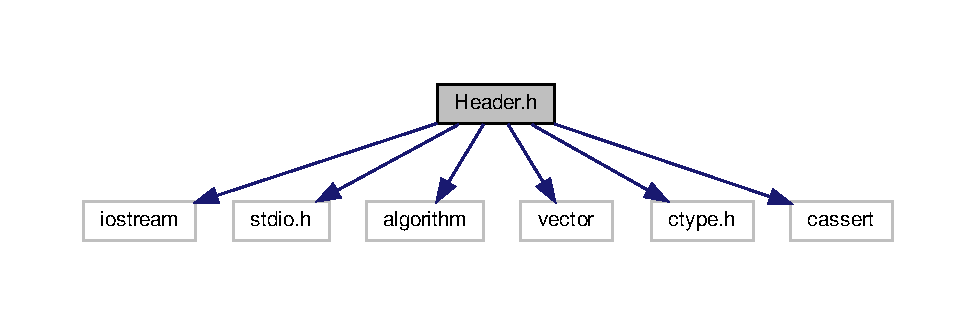
\includegraphics[width=350pt]{_header_8h__incl}
\end{center}
\end{figure}
\subsection*{Classes}
\begin{DoxyCompactItemize}
\item 
struct \hyperlink{struct_opened_string}{Opened\+String}
\begin{DoxyCompactList}\small\item\em Structure that allows you to use itself as a string without storing a buffer. \end{DoxyCompactList}\end{DoxyCompactItemize}
\subsection*{Functions}
\begin{DoxyCompactItemize}
\item 
\mbox{\Hypertarget{_header_8h_a6b3623ca2e4017f351a929e026b0730a}\label{_header_8h_a6b3623ca2e4017f351a929e026b0730a}} 
void {\bfseries Print\+String} (const \hyperlink{struct_opened_string}{Opened\+String} $\ast$string, F\+I\+LE $\ast$output)
\item 
void \hyperlink{_header_8h_a322ee2be66125a40bd235924713813cd}{Shift\+To\+End} (\hyperlink{struct_opened_string}{Opened\+String} $\ast$string)
\begin{DoxyCompactList}\small\item\em Shifts the string pointer to the last character of the string. \end{DoxyCompactList}\item 
\mbox{\Hypertarget{_header_8h_aa16c4bcfd2283c11af1761bce011f915}\label{_header_8h_aa16c4bcfd2283c11af1761bce011f915}} 
void {\bfseries Shift\+To\+End\+In\+Array} (\hyperlink{struct_opened_string}{Opened\+String} $\ast$strings, size\+\_\+t len)
\item 
void \hyperlink{_header_8h_a912c007df89c224fb6baf31ac3ad2715}{Shift\+To\+Begin} (\hyperlink{struct_opened_string}{Opened\+String} $\ast$string)
\begin{DoxyCompactList}\small\item\em Similar to \hyperlink{_header_8h_a322ee2be66125a40bd235924713813cd}{Shift\+To\+End()}, but shifts the pointer to the first character. \end{DoxyCompactList}\item 
\mbox{\Hypertarget{_header_8h_a94bdd388e19d6415909d0e2d576c7959}\label{_header_8h_a94bdd388e19d6415909d0e2d576c7959}} 
void {\bfseries Shift\+To\+Begin\+In\+Array} (\hyperlink{struct_opened_string}{Opened\+String} $\ast$strings, size\+\_\+t len)
\item 
\mbox{\Hypertarget{_header_8h_a2826d8e5541b0e2ae744a173fdfeddfd}\label{_header_8h_a2826d8e5541b0e2ae744a173fdfeddfd}} 
void {\bfseries Print\+Buffer} (const char $\ast$buffer, size\+\_\+t size, F\+I\+LE $\ast$output)
\item 
void \hyperlink{_header_8h_aaf715d07adcfb11fc12d56ad74119f3c}{Sort\+Strings\+In\+Order} (F\+I\+LE $\ast$input, F\+I\+LE $\ast$output)
\begin{DoxyCompactList}\small\item\em Sorts strings from input file and writes sorted strings to output file. Sorts from the beginning of lines firstly, then from the end. \end{DoxyCompactList}\item 
void \hyperlink{_header_8h_a4a86431cb465dd0176d3b686c20628d6}{Write\+To\+File} (const \hyperlink{struct_opened_string}{Opened\+String} $\ast$strings, size\+\_\+t size, F\+I\+LE $\ast$output)
\begin{DoxyCompactList}\small\item\em Writes to file an array of strings. \end{DoxyCompactList}\item 
\mbox{\Hypertarget{_header_8h_afc4cb5735bed6d2f725543a767e7a6f3}\label{_header_8h_afc4cb5735bed6d2f725543a767e7a6f3}} 
int {\bfseries Cmp} (const void $\ast$farg, const void $\ast$sarg)
\item 
int \hyperlink{_header_8h_a9919a3f927f88676ebe297545c67a642}{Get\+Sign} (const int \&number)
\begin{DoxyCompactList}\small\item\em Returns the sign of a number. \end{DoxyCompactList}\item 
\mbox{\Hypertarget{_header_8h_ab252aacdfd5760381413e9077eca62f8}\label{_header_8h_ab252aacdfd5760381413e9077eca62f8}} 
size\+\_\+t {\bfseries Count\+Strings} (char $\ast$buffer, size\+\_\+t $\ast$len)
\item 
\mbox{\Hypertarget{_header_8h_ab1c11f2be92f920055e61dd0bff5879f}\label{_header_8h_ab1c11f2be92f920055e61dd0bff5879f}} 
size\+\_\+t {\bfseries Count\+File\+Size} (F\+I\+LE $\ast$file\+\_\+ptr)
\item 
\hyperlink{struct_opened_string}{Opened\+String} $\ast$ \hyperlink{_header_8h_aeace3eaf4143d54869d7ff6e206ca85f}{Read\+Strings} (char $\ast$buffer, size\+\_\+t $\ast$len)
\begin{DoxyCompactList}\small\item\em Reads strings from buffer. \end{DoxyCompactList}\item 
\mbox{\Hypertarget{_header_8h_a3be2fcde92ade6a8a465fa6514bce26b}\label{_header_8h_a3be2fcde92ade6a8a465fa6514bce26b}} 
bool {\bfseries Is\+Letter} (const char $\ast$symbol)
\item 
char $\ast$ \hyperlink{_header_8h_a67251695223c5ab12f14df913ffb0213}{Read\+Buffer} (F\+I\+LE $\ast$file\+\_\+ptr, size\+\_\+t $\ast$len)
\begin{DoxyCompactList}\small\item\em Reads buffer from file. \end{DoxyCompactList}\end{DoxyCompactItemize}


\subsection{Function Documentation}
\mbox{\Hypertarget{_header_8h_a9919a3f927f88676ebe297545c67a642}\label{_header_8h_a9919a3f927f88676ebe297545c67a642}} 
\index{Header.\+h@{Header.\+h}!Get\+Sign@{Get\+Sign}}
\index{Get\+Sign@{Get\+Sign}!Header.\+h@{Header.\+h}}
\subsubsection{\texorpdfstring{Get\+Sign()}{GetSign()}}
{\footnotesize\ttfamily int Get\+Sign (\begin{DoxyParamCaption}\item[{const int \&}]{number }\end{DoxyParamCaption})}



Returns the sign of a number. 


\begin{DoxyParams}[1]{Parameters}
\mbox{\tt in}  & {\em number} & a number, which sign we want to know\\
\hline
\end{DoxyParams}
\begin{DoxyReturn}{Returns}
1 or -\/1 
\end{DoxyReturn}
\mbox{\Hypertarget{_header_8h_a67251695223c5ab12f14df913ffb0213}\label{_header_8h_a67251695223c5ab12f14df913ffb0213}} 
\index{Header.\+h@{Header.\+h}!Read\+Buffer@{Read\+Buffer}}
\index{Read\+Buffer@{Read\+Buffer}!Header.\+h@{Header.\+h}}
\subsubsection{\texorpdfstring{Read\+Buffer()}{ReadBuffer()}}
{\footnotesize\ttfamily char$\ast$ Read\+Buffer (\begin{DoxyParamCaption}\item[{F\+I\+LE $\ast$}]{file\+\_\+ptr,  }\item[{size\+\_\+t $\ast$}]{len }\end{DoxyParamCaption})}



Reads buffer from file. 


\begin{DoxyParams}{Parameters}
{\em file\+\_\+ptr} & is a pointer on a file.\\
\hline
{\em len} & is an amount of symbols.\\
\hline
\end{DoxyParams}
\begin{DoxyReturn}{Returns}
Array of symbols. 
\end{DoxyReturn}
\mbox{\Hypertarget{_header_8h_aeace3eaf4143d54869d7ff6e206ca85f}\label{_header_8h_aeace3eaf4143d54869d7ff6e206ca85f}} 
\index{Header.\+h@{Header.\+h}!Read\+Strings@{Read\+Strings}}
\index{Read\+Strings@{Read\+Strings}!Header.\+h@{Header.\+h}}
\subsubsection{\texorpdfstring{Read\+Strings()}{ReadStrings()}}
{\footnotesize\ttfamily \hyperlink{struct_opened_string}{Opened\+String}$\ast$ Read\+Strings (\begin{DoxyParamCaption}\item[{char $\ast$}]{buffer,  }\item[{size\+\_\+t $\ast$}]{len }\end{DoxyParamCaption})}



Reads strings from buffer. 


\begin{DoxyParams}{Parameters}
{\em buffer} & it is a pointer on buffer.\\
\hline
{\em len} & is an amount of symbols.\\
\hline
\end{DoxyParams}
\begin{DoxyReturn}{Returns}
Array of strings. 
\end{DoxyReturn}
\mbox{\Hypertarget{_header_8h_a912c007df89c224fb6baf31ac3ad2715}\label{_header_8h_a912c007df89c224fb6baf31ac3ad2715}} 
\index{Header.\+h@{Header.\+h}!Shift\+To\+Begin@{Shift\+To\+Begin}}
\index{Shift\+To\+Begin@{Shift\+To\+Begin}!Header.\+h@{Header.\+h}}
\subsubsection{\texorpdfstring{Shift\+To\+Begin()}{ShiftToBegin()}}
{\footnotesize\ttfamily void Shift\+To\+Begin (\begin{DoxyParamCaption}\item[{\hyperlink{struct_opened_string}{Opened\+String} $\ast$}]{string }\end{DoxyParamCaption})}



Similar to \hyperlink{_header_8h_a322ee2be66125a40bd235924713813cd}{Shift\+To\+End()}, but shifts the pointer to the first character. 


\begin{DoxyParams}{Parameters}
{\em string} & is a pointer on a string, which pointer we want to shift. \\
\hline
\end{DoxyParams}
\mbox{\Hypertarget{_header_8h_a322ee2be66125a40bd235924713813cd}\label{_header_8h_a322ee2be66125a40bd235924713813cd}} 
\index{Header.\+h@{Header.\+h}!Shift\+To\+End@{Shift\+To\+End}}
\index{Shift\+To\+End@{Shift\+To\+End}!Header.\+h@{Header.\+h}}
\subsubsection{\texorpdfstring{Shift\+To\+End()}{ShiftToEnd()}}
{\footnotesize\ttfamily void Shift\+To\+End (\begin{DoxyParamCaption}\item[{\hyperlink{struct_opened_string}{Opened\+String} $\ast$}]{string }\end{DoxyParamCaption})}



Shifts the string pointer to the last character of the string. 


\begin{DoxyParams}{Parameters}
{\em string} & is a pointer on a string, which pointer we want to shift. \\
\hline
\end{DoxyParams}
\mbox{\Hypertarget{_header_8h_aaf715d07adcfb11fc12d56ad74119f3c}\label{_header_8h_aaf715d07adcfb11fc12d56ad74119f3c}} 
\index{Header.\+h@{Header.\+h}!Sort\+Strings\+In\+Order@{Sort\+Strings\+In\+Order}}
\index{Sort\+Strings\+In\+Order@{Sort\+Strings\+In\+Order}!Header.\+h@{Header.\+h}}
\subsubsection{\texorpdfstring{Sort\+Strings\+In\+Order()}{SortStringsInOrder()}}
{\footnotesize\ttfamily void Sort\+Strings\+In\+Order (\begin{DoxyParamCaption}\item[{F\+I\+LE $\ast$}]{input,  }\item[{F\+I\+LE $\ast$}]{output }\end{DoxyParamCaption})}



Sorts strings from input file and writes sorted strings to output file. Sorts from the beginning of lines firstly, then from the end. 


\begin{DoxyParams}{Parameters}
{\em input} & is a pointer on input file.\\
\hline
{\em output} & is a pointer on output file. \\
\hline
\end{DoxyParams}
\mbox{\Hypertarget{_header_8h_a4a86431cb465dd0176d3b686c20628d6}\label{_header_8h_a4a86431cb465dd0176d3b686c20628d6}} 
\index{Header.\+h@{Header.\+h}!Write\+To\+File@{Write\+To\+File}}
\index{Write\+To\+File@{Write\+To\+File}!Header.\+h@{Header.\+h}}
\subsubsection{\texorpdfstring{Write\+To\+File()}{WriteToFile()}}
{\footnotesize\ttfamily void Write\+To\+File (\begin{DoxyParamCaption}\item[{const \hyperlink{struct_opened_string}{Opened\+String} $\ast$}]{strings,  }\item[{size\+\_\+t}]{size,  }\item[{F\+I\+LE $\ast$}]{output }\end{DoxyParamCaption})}



Writes to file an array of strings. 


\begin{DoxyParams}{Parameters}
{\em strings} & it is a pointer on an array of strings.\\
\hline
{\em size} & is an amount of strings.\\
\hline
{\em output} & is a pointer on file to write. \\
\hline
\end{DoxyParams}

%--- End generated contents ---

% Index
\backmatter
\newpage
\phantomsection
\clearemptydoublepage
\addcontentsline{toc}{chapter}{Index}
\printindex

\end{document}
